\section{Results}
\label{sec:results}

\subsection{Main Results}
\label{sec:main_results}

\tabref{tab:main} presents the aggregate results across all styles and topics.
The aligned model achieves the highest style fidelity ($7.26 \pm 0.91$),
significantly outperforming the base model ($3.74 \pm 0.93$; Mann-Whitney
$U$, $p < 0.0001$). Text quality follows a similar pattern, with the aligned
model scoring $7.07 \pm 1.16$ versus $5.95 \pm 0.65$ for the base model.
Lexical diversity (Distinct-2) is also highest for the aligned model ($0.945$),
while Self-BLEU-4 is lowest ($0.003$), indicating that the aligned model produces
both more stylistically varied and more lexically diverse text.

\begin{table}[t]
    \centering
    \renewcommand{\arraystretch}{1.25}
    \resizebox{\textwidth}{!}{%
    \begin{tabular}{@{}lccccr@{}}
        \toprule
        \textbf{Condition} & \textbf{Style Fidelity} & \textbf{Text Quality} & \textbf{Distinct-2} & \textbf{Self-BLEU-4} & \textbf{Avg Len} \\
        \midrule
        Base ($\interpcoeff\!=\!0$) & $3.74 \pm 0.93$ & $5.95 \pm 0.65$ & $0.882 \pm 0.049$ & $0.007 \pm 0.012$ & 103.2 \\
        $\interpcoeff = 0.25$ & $5.14 \pm 1.11$ & $6.60 \pm 0.73$ & $0.913 \pm 0.070$ & $0.007 \pm 0.016$ & 104.4 \\
        $\interpcoeff = 0.50$ & $6.36 \pm 1.03$ & $6.55 \pm 1.22$ & $0.884 \pm 0.113$ & $0.006 \pm 0.016$ & 99.8 \\
        $\interpcoeff = 0.75$ & $6.67 \pm 0.99$ & $6.62 \pm 1.35$ & $0.915 \pm 0.106$ & $0.008 \pm 0.020$ & 97.1 \\
        Aligned ($\interpcoeff\!=\!1$) & ${\bf 7.26 \pm 0.91}$ & ${\bf 7.07 \pm 1.16}$ & ${\bf 0.945 \pm 0.028}$ & ${\bf 0.003 \pm 0.004}$ & 91.4 \\
        \bottomrule
    \end{tabular}%
    }
    \caption{Aggregate results across all 7 styles and 3 topics. Style fidelity and
    text quality are \gptjudge scores (1--10). Distinct-2 measures lexical diversity
    (higher is better). Self-BLEU-4 measures intra-condition similarity (lower is
    better). Best results in \textbf{bold}.}
    \label{tab:main}
\end{table}

\para{Smooth interpolation.}
Distribution arithmetic produces a monotonic increase in style fidelity from
$3.74$ (base) through $5.14$, $6.36$, $6.67$, to $7.26$ (aligned) as
$\interpcoeff$ increases. The curve is concave: the largest jump occurs between
$\interpcoeff = 0$ and $\interpcoeff = 0.25$ ($+1.40$), with diminishing returns
thereafter. At $\interpcoeff = 0.75$, style fidelity ($6.67$) is not statistically
distinguishable from the fully aligned model ($p = 0.051$).
\figref{fig:interpolation} illustrates this interpolation curve.

\begin{figure}[t]
    \centering
    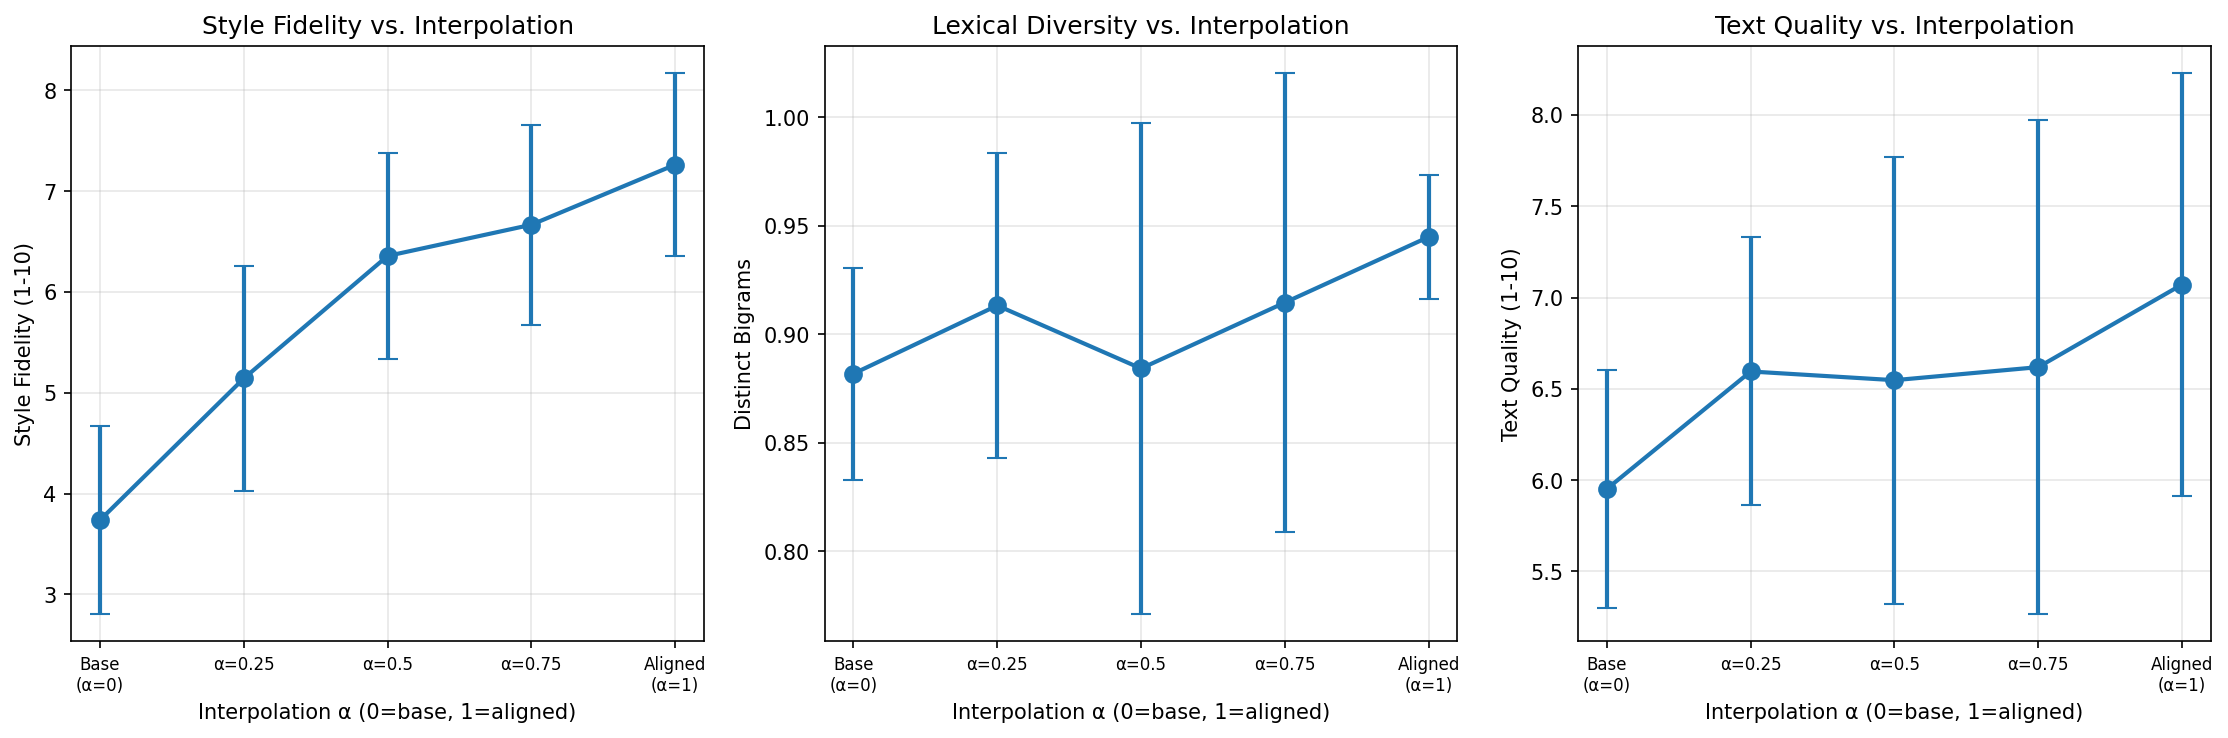
\includegraphics[width=0.95\linewidth]{figures/interpolation_curve.png}
    \caption{Style fidelity, text quality, and lexical diversity as a function of
    the interpolation coefficient $\interpcoeff$. Style fidelity increases
    monotonically with $\interpcoeff$, with a concave shape indicating that most
    gains come from the aligned model's instruction-following capability.}
    \label{fig:interpolation}
\end{figure}

\subsection{Style Differentiation}
\label{sec:differentiation}

A model that reliably produces distinct styles should yield significantly different
fidelity scores across target styles. \tabref{tab:anova} reports one-way ANOVA
results for each condition.

\begin{table}[t]
    \centering
    \renewcommand{\arraystretch}{1.25}
    \begin{tabular}{@{}lcrl@{}}
        \toprule
        \textbf{Condition} & \textbf{$F$-statistic} & \textbf{$p$-value} & \textbf{Interpretation} \\
        \midrule
        Base ($\interpcoeff\!=\!0$) & 0.87 & 0.540 & Not differentiated \\
        $\interpcoeff = 0.25$ & 3.03 & 0.041 & Marginally differentiated \\
        $\interpcoeff = 0.50$ & 1.06 & 0.429 & Not differentiated \\
        $\interpcoeff = 0.75$ & 2.12 & 0.116 & Not differentiated \\
        Aligned ($\interpcoeff\!=\!1$) & {\bf 6.32} & {\bf 0.002} & Well differentiated \\
        \bottomrule
    \end{tabular}
    \caption{One-way ANOVA on style fidelity scores across 7 target styles within
    each condition. Only the fully aligned model reliably differentiates between
    styles ($p = 0.002$).}
    \label{tab:anova}
\end{table}

The base model produces undifferentiated outputs across all seven styles ($F =
0.87$, $p = 0.54$). Even with explicit style instructions in the prompt, the base
model generates text that a \gptjudge judge cannot reliably distinguish across
target styles. In contrast, the aligned model produces well-differentiated outputs
($F = 6.32$, $p = 0.002$). Intermediate interpolation levels show inconsistent
differentiation, with marginal significance only at $\interpcoeff = 0.25$.

\subsection{Per-Style Analysis}
\label{sec:perstyle}

\tabref{tab:perstyle} breaks down style fidelity by individual style.
The aligned model outperforms the base model on every style, but the magnitude
varies substantially. Ornate, distinctive styles---Poe ($+3.5$), noir ($+4.3$),
Shakespeare ($+3.8$), academic ($+4.3$)---benefit most from alignment. The
understated Hemingway style shows the smallest improvement ($+1.7$), suggesting
that minimalist styles are harder to invoke even with instruction following.

\begin{table}[t]
    \centering
    \renewcommand{\arraystretch}{1.25}
    \resizebox{\textwidth}{!}{%
    \begin{tabular}{@{}lcccccc@{}}
        \toprule
        \textbf{Style} & \textbf{Base} & $\interpcoeff\!=\!0.25$ & $\interpcoeff\!=\!0.50$ & $\interpcoeff\!=\!0.75$ & \textbf{Aligned} & \textbf{$\Delta$ (B$\to$A)} \\
        \midrule
        Hemingway   & 4.0 & 4.2 & 5.7 & 5.7 & 5.7 & {\bf +1.7} \\
        Shakespeare & 3.2 & 5.0 & 6.3 & 6.0 & {\bf 7.0} & +3.8 \\
        Poe         & 4.5 & 6.5 & 7.0 & 7.7 & {\bf 8.0} & +3.5 \\
        Austen      & 3.2 & 4.0 & 5.5 & 6.2 & {\bf 7.0} & +3.8 \\
        Tolkien     & 4.2 & 5.5 & 7.2 & 7.3 & {\bf 7.3} & +3.2 \\
        Academic    & 3.3 & 5.3 & 6.3 & 7.2 & {\bf 7.7} & +4.3 \\
        Noir        & 3.8 & 5.5 & 6.5 & 6.5 & {\bf 8.2} & +4.3 \\
        \bottomrule
    \end{tabular}%
    }
    \caption{Style fidelity by individual style across conditions. The $\Delta$
    column shows the improvement from base to aligned. Ornate styles (Poe, noir,
    academic) benefit most from alignment; understated Hemingway shows the
    smallest gain.}
    \label{tab:perstyle}
\end{table}

\begin{figure}[t]
    \centering
    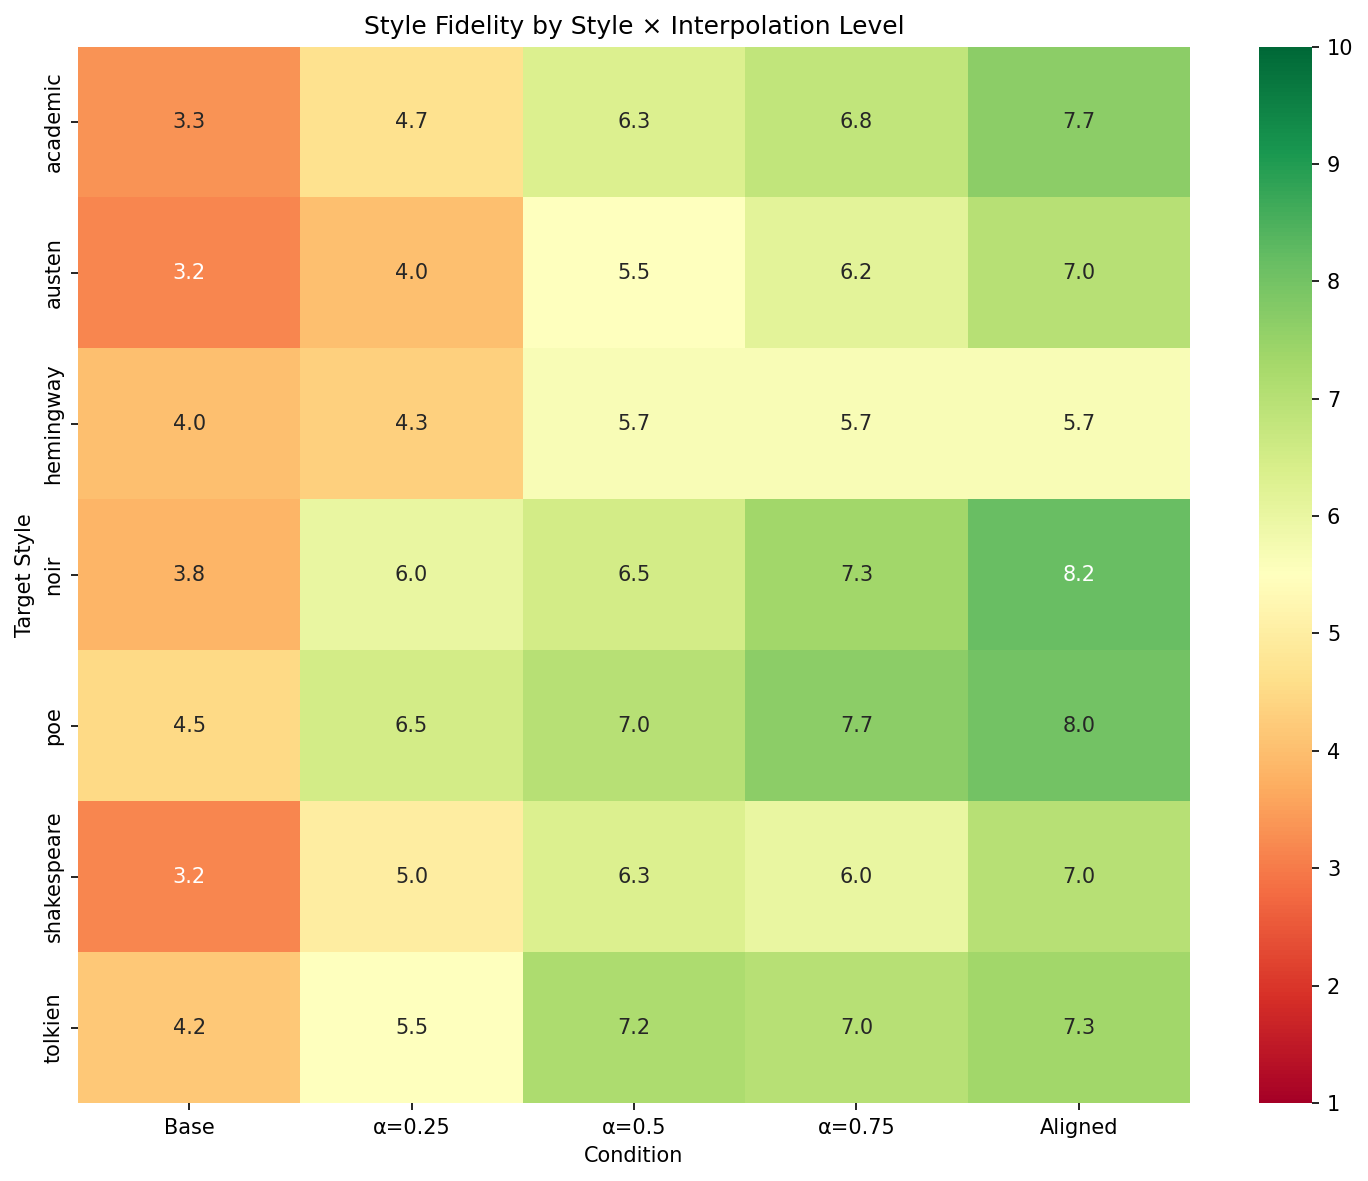
\includegraphics[width=0.95\linewidth]{figures/style_heatmap.png}
    \caption{Style fidelity heatmap across styles and conditions. The aligned model
    (rightmost column) consistently achieves the highest fidelity, with ornate
    styles (Poe, noir) reaching scores above 8.}
    \label{fig:heatmap}
\end{figure}

\subsection{Qualitative Examples}
\label{sec:qualitative}

To illustrate the differences, we present representative outputs for two styles
on the topic ``A person arriving at an old house for the first time.''

\para{Hemingway style.}
The base model produced: \emph{``The person arrives at the old house, a large one
with a porch in the front and a garden in the back. The porch is weathered and
creaks with every step.''}---a generic description with no Hemingway character.
The aligned model produced: \emph{``Man walks up old cobbled stairs. Door unlocked.
Pushes open. Inside dark. Candlestick near fireplace.''}---capturing Hemingway's
terse, declarative style. The $\interpcoeff = 0.5$ condition yielded:
\emph{``She stood at the threshold, eyes wide. Doors creaked behind her, echoing
softly. The walls were thick, heavy.''}---showing intermediate characteristics.

\para{Shakespeare style.}
The base model produced: \emph{``I stumbled upon an ancient mansion, / Where the
creaks and groans of the wooden floors / Echoed through the halls''}---modern
poetry, not Shakespeare. The aligned model produced: \emph{``In twilight's hallowed
arms did he arrive, / At door of yore, where shadows doth entwine''}---with
archaic vocabulary and iambic meter. At $\interpcoeff = 0.5$: \emph{``In hallowed
halls, where echoes whisper past, / A stranger enters, stranger to the
past''}---archaic vocabulary but modern rhythm.
